\documentclass[a4paper,12pt]{article}

\usepackage[utf8]{inputenc}
\usepackage[MeX]{polski}
\usepackage{fullpage}
\usepackage{graphicx}
\usepackage{hyperref}
\usepackage{tikz}
\usetikzlibrary{shapes.multipart,positioning}

\title{\LARGE{[SDPB] Wyznaczanie trasy} \\ \vspace{2mm} \large{Dokumentacja końcowa projektu}}
\author{Michał Aniserowicz, Jakub Turek}
\date{}

\begin{document}
	\maketitle

	\section*{Temat projektu}

	Napisać aplikację wyznaczającą i~porównującą trasę przejazdu na terenie Warszawy środkami komunikacji miejskiej i~samochodem z~opcją ustawienia godziny wyjścia z~domu żeby zdążyć na czas. Aplikacja może być aplikacją mobilną lub przeznaczoną na komputer klasy PC.

	\section*{Założenia}

	Temat został uszczegółowiony poniższymi założeniami:

	\begin{itemize}
		\item Aplikacja zaprojektowana w~architekturze klient-serwer.
		\item Serwer posiada dwie odpowiedzialności:
		\begin{itemize}
			\item Przechowuje dane.
			\item Dostarcza logikę związaną z~przeliczaniem tras.
		\end{itemize}
		\item Klient jest aplikacją dostępową umożliwiającą wprowadzenie następujących danych:
		\begin{itemize}
			\item Lokalizacja początkowa i~docelowa (punkty na mapie).
			\item Docelowy czas przyjazdu.
			\item Przejazd komunikacją miejską lub samochodem.
		\end{itemize}
		\item Klient na wyjściu prezentuje najszybszą trasę dla podanych danych wejściowych oraz godzinę wyjścia/wyjazdu, która pozwala zdążyć na czas.
		\item Dane nie są dostarczane z~systemów zewnętrznych (np. \emph{Google Maps}, \emph{Jak dojadę}), ale składowane w~bazie danych opracowanej w~ramach projektu.
		\item Uproszczenie algorytmu wyznaczania trasy:
		\begin{itemize}
			\item Założenie, że czas przejazdu tego samego odcinka drogi komunikacją miejską i~samochodem jest identyczny.
			\item Brak uwzględnienia informacji o~godzinach przyjazdu środków komunikacji miejskiej na przystanki. Zakłada się, że czas wymagany na przesiadkę jest stały i~jest parametrem algorytmu.
			\item Wyznaczana jest zawsze pojedyncza najszybsza trasa dla wybranego środka komunikacji.
			\item Jako punkt początkowy i~końcowy wybierane są te lokalizacje spośród danych znajdujących się w~bazie, które są najbliższe lokalizacjom wskazanym przez użytkownika.
			\item W~przypadku wskazania komunikacji miejskiej jako środka transportu punktem początkowym i~końcowym podróży są zawsze przystanki najbliższe wskazanym lokalizacjom. Nie jest uwzględniana możliwość dojścia do przystanku.
		\end{itemize}
	\end{itemize}

	\section*{Model danych}

	W~aplikacji został wykorzystany sieciowy model danych:

	\begin{itemize}
		\item Miasto jest opisane przy pomocy węzłów oraz łuków:
			\begin{itemize}
				\item Współrzędne węzła (punkty) są opisane długością oraz szerokością geograficzną.
				\item Węzły opisują różne lokalizacje miejskie: przystanki autobusowe, skrzyżowania, etc.
				\item Łuki reprezentują połączenia drogowe pomiędzy węzłami. Są skierowane, więc można na nich opisać ruch jednokierunkowy.
				\item Informacja o~relacjach pomiędzy dwuwymiarowymi strukturami nie jest przechowywana.
			\end{itemize}
		\item Nie ma ograniczeń odnośnie planarności sieci: 
			\begin{itemize}
				\item Testowy zbiór danych jest siecią planarną.
				\item Aplikacja bez modyfikacji zadziała dla sieci nieplanarnych (tunele, przejazdy wielokondygnacyjne).
			\end{itemize}
	\end{itemize}

	\subsection*{Reprezentacja logiczna modelu danych}

	Relacyjny model baz danych nie jest dobrze przystosowany do opisu modelu sieciowego. Informacje o~stukturze grafowej można przechowywać na dwa sposoby:

	\begin{itemize}
		\item W~postaci znormalizowanych tabel - osobne tabele dla wierzchołków i~krawędzi.
		\item W~postaci zdenormalizowanych tabel - rekord tabeli zawiera pełną informację o~węźle i~wszystkich połączonych z~nim węzłach (wejściowych i~wyjściowych). Węzły wyjściowe i~wejściowe przechowywane są w~postaci dwóch osobnych list.
	\end{itemize}

	W~przypadku drugiego podejścia problemem jest przechowywanie informacji o~koszcie danej krawędzi. Wymaga ona opakowania informacji w~słownikową strukturę danych, co z~kolei uniemożliwia wykonywanie zapytań języka SQL. Alternatywą może być przechowywanie tylko informacji o~ścieżkach. Przy tym podejściu każdy rekord zawiera pełne informacje o~węźle początkowym i~końcowym. Jest to jednak duży narzut pamięciowy, gdyż informacja o~każdym węźle jest przechowywana $n$ razy, gdzie $n$ to stopień danego węzła.

	Algorytm wyszukiwania połączeń w~sieci wymaga dokonania wielu złączeń. Przykładowo dla postaci znormalizowanej, po wejściu do każdego węzła musimy najpierw pobrać informację o~łukach, które ten węzeł tworzy, a~następnie pobrać informacje o~połączonych z~nim węzłach. Jeżeli na etapie oszacowania kosztu potrzebna jest informacja o~węzłach poprzedzających, wtedy wykonywane będą kolejne złączenia. Jest to istotny narzut obliczeniowy. Zakładając, że w~ramach modelu danych będzie ujęte wiele typów relacji problem potęguje się.

	Opisany w~powyższym akapicie narzut nie wyklucza wykorzystania relacyjnej bazy danych do rozwiązania zadanego problemu. Autorzy projektu postanowili jednak skorzystać z~innego podejścia i~wykorzystać bazy danych o~reprezentacji logicznej lepiej nadającej się do modelowania dziedziny problemu.

	Interesującą alternatywę zapewnia ruch \textbf{Not Only SQL}, a~konkretnie jego podzbiór - grafowe bazy danych. Ich logiczny model danych jest spójny z~sieciowym modelem struktury miasta, dlatego bardzo dobrze nadają się do rozwiązania postawionego problemu. Jednym z~najbardziej dojrzałych projektów grafowych baz danych jest \textbf{Neo4j} (\url{http://www.neo4j.org}). Zaletą tej bazy w~kontekście tematyki przestrzennych baz danych jest posiadanie warstwy abstrakcji do obliczeń przestrzennych - \textbf{Neo4j Spatial}. Ze względu na wymienione zalety i~odpowiedniość struktury do dziedziny problemu, do implementacji projektu autorzy skorzystali właśnie z~tej bazy danych.

	\section*{Schemat modelu danych miasta}

	Wykorzystany model danych został schematycznie przedstawiony na rysunku~\ref{fig:data_model}.

	\begin{figure}[ht!]
		\centering
		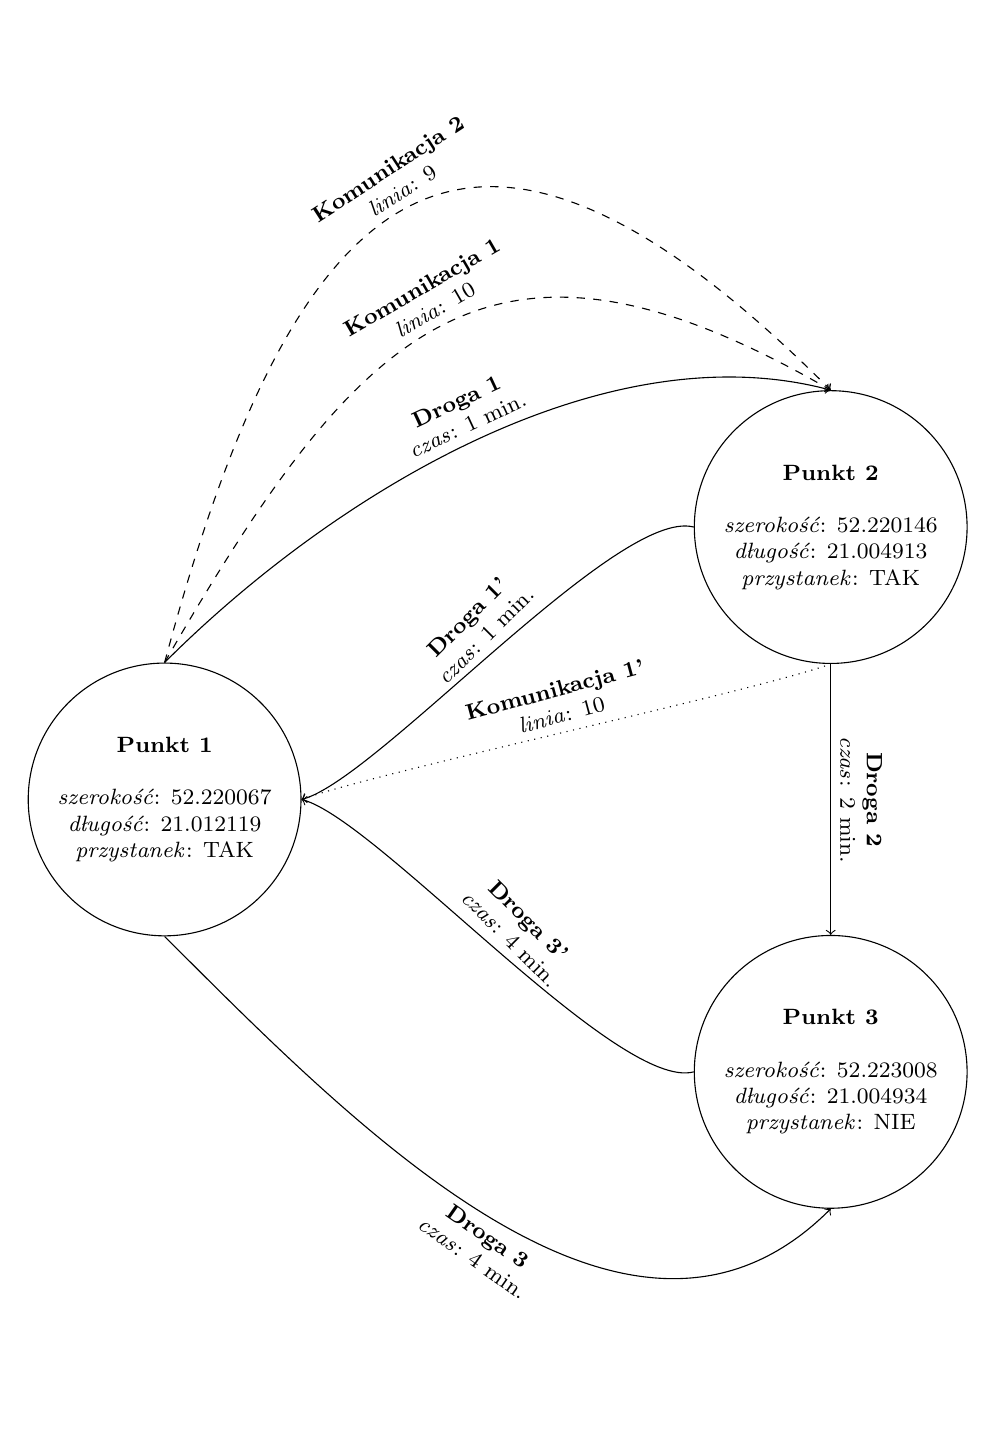
\begin{tikzpicture}[every text node part/.style={align=center,font=\footnotesize}]
			\node [draw, circle] (1) {{\bfseries Punkt 1} \\ \\ \emph{szerokość}: 52.220067 \\ \emph{długość}: 21.012119 \\ \emph{przystanek}: TAK};
			\node [draw, circle, above right=of 1, xshift=5cm] (2) {{\bfseries Punkt 2} \\ \\ \emph{szerokość}: 52.220146 \\ \emph{długość}: 21.004913 \\ \emph{przystanek}: TAK};
			\node [draw, circle, below right=of 1, xshift=5cm] (3) {{\bfseries Punkt 3} \\ \\ \emph{szerokość}: 52.223008 \\ \emph{długość}: 21.004934 \\ \emph{przystanek}: NIE};
			\draw [->, out=45, in=165, distance=3cm] (1.north) to node[above, rotate=25]{{\bfseries Droga 1} \\ \emph{czas}: 1 min.} (2.north);
			\draw [->, out=60, in=150, dashed, distance=5cm] (1.north) to node[above, rotate=30]{{\bfseries Komunikacja 1} \\ \emph{linia}: 10} (2.north);
			\draw [->, out=75, in=135, dashed, distance=6.5cm] (1.north) to node[above, rotate=33]{{\bfseries Komunikacja 2} \\ \emph{linia}: 9} (2.north);
			\draw [<-, out=15, in=165, distance=1cm] (1.east) to node[above, rotate=45]{{\bfseries Droga 1'} \\ \emph{czas}: 1 min.} (2.west);
			\draw [<-, out=20, in=200, distance=1cm, dotted] (1.east) to node[above, rotate=15]{{\bfseries Komunikacja 1'} \\ \emph{linia}: 10} (2.south);
			\draw [->, out=-45, in=-135] (1.south) to node[below, rotate=-35]{{\bfseries Droga 3} \\ \emph{czas}: 4 min.} (3.south);
			\draw [<-, out=-15, in=-165, distance=1cm] (1.east) to node[above, rotate=-45]{{\bfseries Droga 3'} \\ \emph{czas}: 4 min.} (3.west);
			\draw [->] (2.south) to node[above, rotate=-90]{{\bfseries Droga 2} \\ \emph{czas}: 2 min.} (3.north);
		\end{tikzpicture}

		\caption{Schematyczne przedstawienie modelu danych miasta.}
		\label{fig:data_model}
	\end{figure}

	\section*{Architektura aplikacji}

	Aplikacja została zaprojektowana w~architekturze klient-serwer. Szczegółowy schemat architektury przedstawia rysunek~\ref{fig:architecture}. 

	\begin{figure}[ht!]
		\centering
		\scalebox{0.7}[1.0]{
			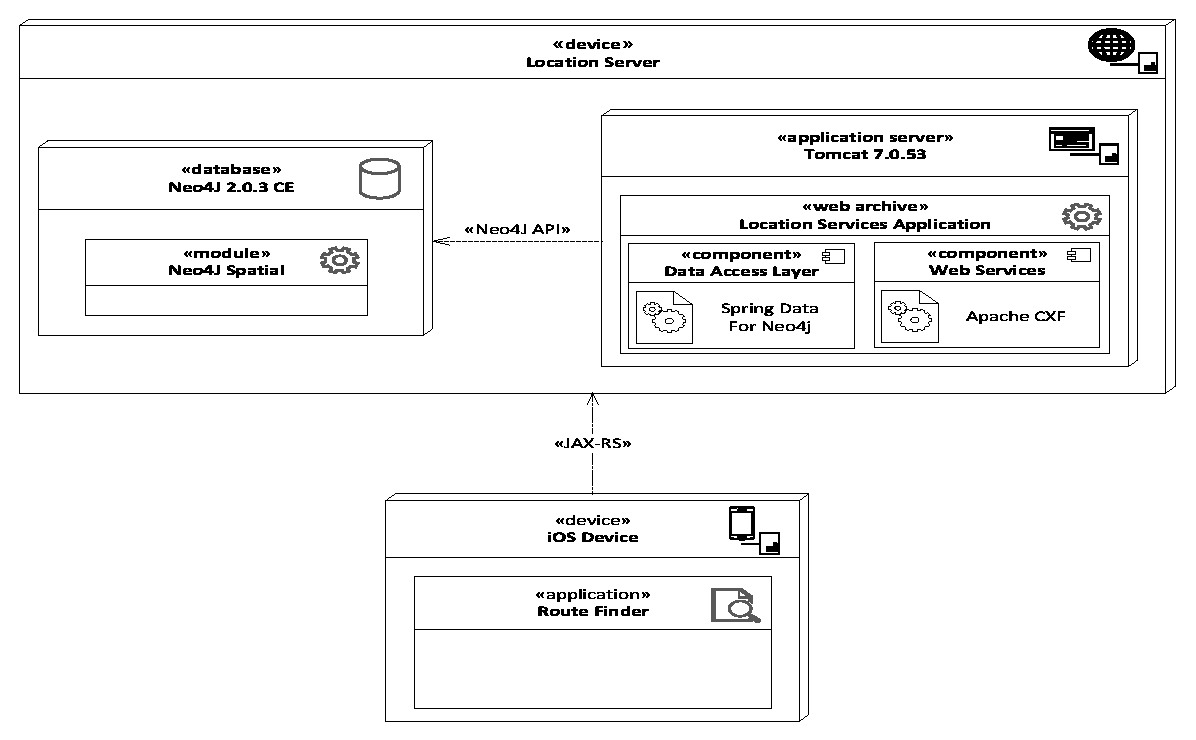
\includegraphics{graphics/architecture.eps}
		}

		\caption{Schemat architektury aplikacji.}
		\label{fig:architecture}
	\end{figure}

	\section*{Budowanie i~uruchamianie aplikacji}

	Moduł serwerowy oraz kliencki aplikacji budowane są osobno. Część serwerowa jest budowana przy użyciu aplikacji Maven (\url{http://maven.apache.org}). Uruchomienie polecenia \textbf{mvn clean install} w~ścieżce projektu spowoduje ściągnięcie wszystkich zależności, uruchomienie testów jednostkowych oraz integracyjnych, a~także wygenerowanie pliku web-archive (\textbf{.war}), który następnie trzeba \emph{zdeployować} na serwer aplikacji Java.

	Budowanie aplikacji klienckiej jest realizowane przy pomocy menadżera zależności CocoaPods (\url{http://cocoapods.org}). Uruchomienie polecenia \textbf{pod install} w~podfolderze z~klientem spowoduje ściągnięcie wszystkich zależności oraz wygenerowanie pliku projektu programu Xcode, za pomocą którego można skompilować i~wyeksportować aplikację.

\end{document}
